\section{Statistical analysis of survey answers}

ANOVA, also known as, analysis of variance, was used to test the hypothesis that the different surveyed groups had different opinions. A similar use to this work` approach is found in \cite{ismail2007organizational}. They used ANOVA to analyze the results of a survey with three different groups of knowledge. This analysis has only two groups, but it not imply in a big change to the model.

The sole purpose of ANOVA is to test the hypothesis that from different group of samples for the same factor have a statistically significant difference in results. This will give the information needed to establish the correct average values for the concepts. Subsequently determining the dynamics which will compose OntoBG-D.

\subsection{Using ANOVA}

Using the ANOVA test require to first test an important hypothesis of the model. The variances of the residues must be equal for the one-way test to work. Test results are displayed in \autoref{fig:anovatest}. With a precision of 95\% the variances are equal and the model can be used. This is due to the p-value being above the confidance interval for both methods of testing. 
\begin{figure}[h!]
    \centering
    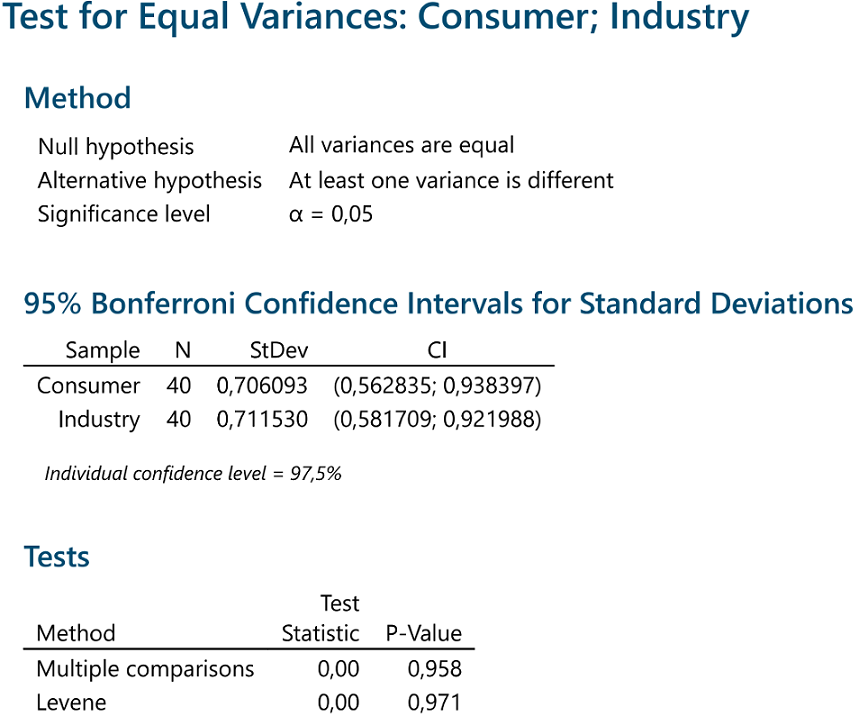
\includegraphics[width=\textwidth]{Images/ANOVA/ANOVATESTENG.png}
    \caption{}
    \label{fig:anovatest}
\end{figure}



\subsection{Analyzing the output}


%\includegraphics[width=\textwidth]{Images/ANOVA/ANOVARESULT.png}